%
% main.tex -- Paper zum Thema <geodaeten>
%
% (c) 2020 Autor, OST Ostschweizer Fachhochschule
%
% !TEX root = ../../buch.tex
% !TEX encoding = UTF-8
%
\chapter{Geodäten\label{chapter:geodaeten}}
\kopflinks{Geodäten}
\begin{refsection}
\chapterauthor{Andrin Kälin}

Ein paar Hinweise für die korrekte Formatierung des Textes
\begin{itemize}
\item
Absätze werden gebildet, indem man eine Leerzeile einfügt.
Die Verwendung von \verb+\\+ ist nur in Tabellen und Arrays gestattet.
\item
Die explizite Platzierung von Bildern ist nicht erlaubt, entsprechende
Optionen werden gelöscht. 
Verwenden Sie Labels und Verweise, um auf Bilder hinzuweisen.
\item
Beginnen Sie jeden Satz auf einer neuen Zeile. 
Damit ermöglichen Sie dem Versionsverwaltungssysteme, Änderungen
in verschiedenen Sätzen von verschiedenen Autoren ohne Konflikt 
anzuwenden.
\item 
Bilden Sie auch für Formeln kurze Zeilen, einerseits der besseren
Übersicht wegen, aber auch um GIT die Arbeit zu erleichtern.
\end{itemize}
Geodätenlinien beschreiben den kürzesten Weg zwischen zwei Punkten auf einer beliebigen Oberfläche.
Dabei ist sowohl Form als auch Dimension beliebig.
Um diese Linien zu berechnen wird das Standardverfahren für Geodätenlinein verwendet, welches auf dem metrischen Tensor des zu untersuchenden Raumes basiert.
Um den Metrischen Tensor aufstellen zu können, müssen zunächst die Linienelemente bekannt sein.
Die folgenden zwei Kapitel sollen zunächst die Linienelemente (Abschnitt \ref{geodaeten:section:Linienelemente}) und den metrischen Tensor (Abschnitt [\ref{geodaeten:section:MetrischerTensor}]) erklären.
Erst dann kann das Standardverfahren anhand einiger Beispiele(Abschnitt \ref{geodaeten:section:StandardverfahrenBeispiele}) veranschaulicht werden.

%
% einleitung.tex -- Beispiel-File für die Einleitung
%
% (c) 2020 Prof Dr Andreas Müller, Hochschule Rapperswil
%
% !TEX root = ../../buch.tex
% !TEX encoding = UTF-8
%
\section{Linienelemente\label{geodaeten:section:Linienelemente}}
\rhead{Linienelemente}

Um die Weglänge unserer Geodätenlinie minimieren zu können, müssen wir erst einmal den Weg berechnen.
Jeder Weg kann in kleinere Wegstücke $\Delta \text{Weg}$ unterteilt werden, welche addiert wieder den ganzen Weg ergeben.
Der Weg $l$ entspricht 
\begin{equation}
	l = \sum \Delta \text{Weg} .
\end{equation}

Linienelemente sind als infinitesimal kleine Wegstücke definiert, welche entlang jeder Dimension integriert die Weglänge ergeben.
Ein Linienelement entlang einer Dimensions-Achse beschreibt, wie sich der Raum in die entsprechende Dimension verändert.
In einem $n$-dimensionalen Raum entspricht ein Linienelement also einem $n$-dimensionalen Vektor, welcher die Kurve in jeder Dimension beschreibt.

Die Wegstücke werden infinitesimal und die Formel für die Wegstücklänge $\Delta \text{Weg}$ wird zur Formel für das Linienelement $ds$  als
\begin{equation}	
	d\text{Weg} = ds .
	\label{geodaeten:equation:Linienelemente:equation1}
\end{equation}

Um den Weg $l$ zu erhalten müssen schliesslich diese Linienelemente in allen Dimensionen integriert werden mit
\begin{equation}
	l = 
	\sum^{n} \int_a^b ds .
	\label{geodaeten:equation:Linienelemente:equation2}
\end{equation}

\section{Beispiele zu Linienelementen\label{geodaeten:section:Linienelemente:Beispiele}}
Die Beispiele sind für alle Abschnitte gleich aufgebaut.
Zuerst wird das zweidimensionale Beispiel des kartesischen Raumes als einfacher Einstieg behandelt.
Danach wird der Zylinder als Übergang in etwas komplexere Strukturen aufgezeigt.
Zum Schluss werden Untersuchungen an einer Kugel durchgeführt, welche in der Praxis grosse Anwendung finden, unter anderem aufgrund der Ähnlichkeit zur Erdkugel (Abbildung \ref{geodaeten:figure:Geodaeten:Erdkugel}).

	%
% einleitung.tex -- Beispiel-File für die Einleitung
%
% (c) 2020 Prof Dr Andreas Müller, Hochschule Rapperswil
%
% !TEX root = ../../buch.tex
% !TEX encoding = UTF-8
%
\subsection{Kartesisch\label{geodaeten:section:LinKartesisch}}
\rhead{Linienelemente Beispiele}

Wie in Abbildung [\ref{geodaeten:Linienelemente:figure1}] zu sehen ist kann ein Wegstück auf einer Kurve im zweidimensionalen Kartesischen Raum mit

\begin{equation}
	\Delta s \approx \sqrt{\Delta x^2 + \Delta y^2}
\end{equation}
approximiert werden.
Durch Verkleinerung der Wegstücke bis zum Infinitesimal 

\begin{equation}
	d s = \sqrt{d x^2 + d y^2}
	= \sqrt{\left(\frac{d x}{d t}\right)^2 \cdot d t^2 + \left(\frac{d y}{d t}\right)^2 \cdot d t^2} ,
\end{equation}
Kann das Linienelement aufgestellt werden als

\begin{equation}
 	ds^2 = \left(\dot{x}^2 +\dot{y}^2\right) \cdot dt^2 .
\end{equation}
Als Vektor dargestellt entspricht das Linienelement

\begin{equation}
	\mathbf{d\vec{s}}^2 = \begin{pmatrix} \dot{x}^2 \\ \dot{y}^2 \end{pmatrix} = \begin{pmatrix} 1 \\ 1 \end{pmatrix} \cdot \begin{pmatrix} \dot{x}^2 \\ \dot{y}^2 \end{pmatrix} \cdot dt^2 .
\end{equation}

\begin{figure}
	\centering
	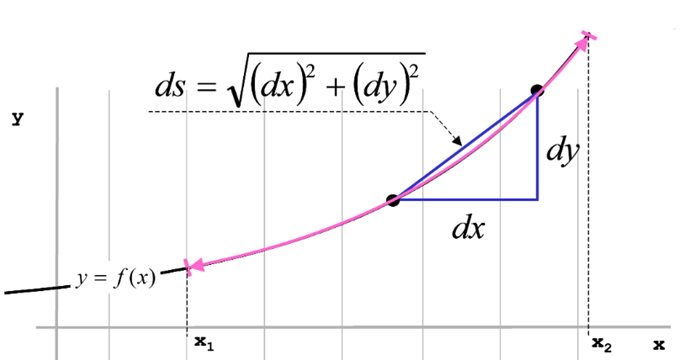
\includegraphics[width=0.7\linewidth]{papers/geodaeten/Abbildungen/Linienelemente/LinKartes1}
	\caption{Linienelement im Kartesischen Raum}
	\label{geodaeten:Linienelemente:figure1}
	\cite{geodaeten:kartesisch}
\end{figure}

	%
% einleitung.tex -- Beispiel-File für die Einleitung
%
% (c) 2020 Prof Dr Andreas Müller, Hochschule Rapperswil
%
% !TEX root = ../../buch.tex
% !TEX encoding = UTF-8
%
\subsection{Zylinder\label{geodaeten:section:Linienelemente:Zylinder}}
\rhead{Linienelemente Beispiele}

Eine Kurve auf der Oberfläche eines Zylinders kann als zweidimensional betrachtet werden, wobei gilt
\begin{equation}
	\Delta s \approx \sqrt{(r \cdot \Delta \phi)^2 + \Delta z^2}
\end{equation}
wenn $r$ konstant ist.
Analog zu den kartesischen Koordinaten können die Abstände infinitesimal werden und das Linienelement ergibt sich dadurch für die Oberfläche des Zylinders zu
\begin{equation}
	ds^2 = r^2 \cdot d \phi^2 + d z^2 .
	\label{geodaeten:equation:Linienelemente:Zylinder:equation2}
\end{equation}

Den Einstieg in dreidimensionale Kurven können wir machen, indem $r$ als nicht konstant angenommen wird.
Der Weg kann so mit
\begin{equation}
	\Delta s \approx \sqrt{\Delta r^2 + (r \cdot \Delta \phi)^2 + \Delta z^2} %\cdot dt^2
\end{equation}
berechnet werden und das Linienelement entspricht 
\begin{equation}
	ds^2 = d r^2 + r^2 \cdot d \phi^2 + d z^2 .
	\label{geodaeten:equation:Linienelemente:Zylinder:Zylinder3D}
\end{equation}

\begin{figure}
	\centering
	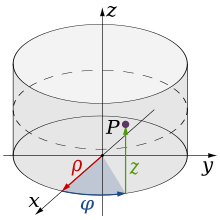
\includegraphics[width=4cm]{papers/geodaeten/Abbildungen/Linienelemente/LinZyl1}
	\caption{zylindrischer Raum mit $r = \rho$. Bildquelle: \cite{geodaeten:polarkoordinaten}}
	\label{geodaeten:figure:Linienelemente:Zylinder:figure2}
	
\end{figure}
	%
% einleitung.tex -- Beispiel-File für die Einleitung
%
% (c) 2020 Prof Dr Andreas Müller, Hochschule Rapperswil
%
% !TEX root = ../../buch.tex
% !TEX encoding = UTF-8
%
\subsection{Kugel\label{geodaeten:section:LinKugel}}
\rhead{Linienelemente Beispiele}

In ähnlicher Weise wie im Beispiel mit dem Zylinder lässt sich eine Kugel lokal wie eine flache Ebene darstellen.
Was auf den ersten Blick für sogenannte "Flat-Earther" ein schwieriges Konzept zu sein scheint, ist intuitiv verständlich:
Zoomt man nahe genug an die Erdoberfläche heran, verschwinden die Krümmungen, und Abstände lassen sich nahezu wie in einem euklidischen Raum berechnen.

In Kugelkoordinaten beschreibt $r$ den Abstand eines Punktes vom Zentrum der Kugel (Radius), $\theta$ den Winkel zur z-Achse (Polarwinkel), und $\phi$ den Winkel in der xy-Ebene (Azimutwinkel).
Diese Parameter definieren die Position eines Punktes auf der Kugeloberfläche eindeutig, wie in der Abbildung dargestellt.

Da wir uns auf der Oberfläche der Kugel befinden, bleibt $r$ konstant, und wir betrachten nur die Winkel $\theta$ und $\phi$.
Wenn ein Punkt nun um einen infinitesimalen Abstand auf der Kugeloberfläche verschoben wird, entstehen Verschiebungen entlang der zugehörigen Basisvektoren:
$r \, d\theta$ für die Breitenrichtung und $r \sin\theta \, d\phi$ für die Längsrichtung.

Weil lokal gerechnet werden kann wie in einem euklidischen Raum, ergibt sich der Abstand zwischen zwei Punkten auf der Kugeloberfläche durch die Anwendung des Pythagoras auf die jeweiligen infinetsimalen Verschiebungen entlang der Basisvektoren.

Das Linienelement $ds$ für die Oberfläche der Kugel kann daher als
\begin{equation}
ds^2 = r^2 \, d\theta^2 + r^2 \, \sin^2\theta \, d\phi^2
\end{equation}
beschrieben werden.

\begin{figure}
	\centering
	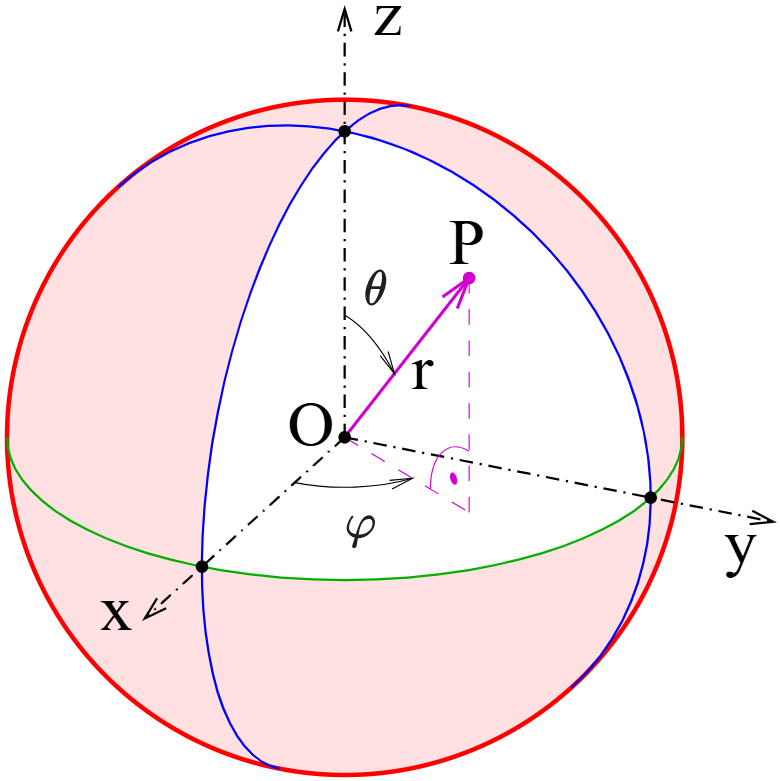
\includegraphics[width=0.7\linewidth]{papers/geodaeten/Abbildungen/Linienelemente/LinKugel1}
	\caption{Kugelkoordinaten mit Radius $r$, Polarwinkel $\theta$ und Azimutwinkel $\phi$}
	\label{geodaeten:figure:Linienelemente:Kugelkoordinaten}
	\cite{geodaeten:Kugelkoordinaten}
\end{figure}



 %
% teil1.tex -- Beispiel-File für das Paper
%
% (c) 2020 Prof Dr Andreas Müller, Hochschule Rapperswil
%
% !TEX root = ../../buch.tex
% !TEX encoding = UTF-8
%
\section{Der Metrische Tensor
\label{geodaeten:section:MetrischerTensor}}
\kopfrechts{Der Metrische Tensor}

Im vorherigen Kapitel wurde das Konzept des Linienelements erläutert.
Es wurde aufgezeigt, wie dieses mittels geometrischer Analyse für verschiedene Räume und Koordinatensysteme berechnet werden kann.
Aus der Vektorgeometrie ist uns jedoch ein anderes nützliches Werkzeug bekannt, welches uns erlaubt, Abstände in einem Raum zu berechnen: Das Skalarprodukt.
\index{Skalarprodukt}%

\subsection{Skalarprodukt im euklidischen Raum}
Im euklidischen Raum ist das Skalarprodukt zwischen zwei Vektoren $\vec{u}$ und $\vec{v}$ definiert als
\begin{equation}
	\vec{u} \cdot \vec{v} = \sum_{i=1}^n u_i v_i,
\end{equation}
wobei $\vec{u} = (u_1, u_2, \ldots, u_n)$ und $\vec{v} = (v_1, v_2, \ldots, v_n)$ die Komponenten der Vektoren in einem $n$-dimensionalen Raum sind.

Die Länge eines Vektors $\vec{u}$ ergibt sich als die Wurzel aus dem Skalarprodukt des Vektors mit sich selbst, also
\begin{equation}
	\|\vec{u}\| = \sqrt{\vec{u} \cdot \vec{u}} = \sqrt{\sum_{i=1}^n u_i^2}.
\end{equation}

Betrachten wir nun einen infinitesimal kleinen Vektor in einer Ebene mit kartesischen Koordinaten $(x, y)$, dann ergibt das Skalarprodukt dieses Vektors mit sich selbst
\begin{equation}
	ds^2 = dx \cdot dx + dy \cdot dy = dx^2 + dy^2,
\end{equation}
was die quadratische infinitesimale Länge des Vektors beschreibt und dem bereits bekannten Linienelement entspricht.

Diese Definition des Skalarprodukts ist jedoch nicht allgemeingültig und gilt nur für die Berechnung von Abständen im euklidischen Raum.
Für komplexere Räume mit speziellen Koordinatensystemen wie Zylinder- oder Kugelkoordinaten müssen wir zuerst die Konzepte der Mannigfaltigkeit und des metrischen Tensors verstehen.

\subsection{Mannigfaltigkeit}
\index{Mannigfaltikgeit}
Eine Mannigfaltigkeit ist ein mathematisches Konstrukt, das dazu dient, komplizierte geometrische Objekte in eine einfachere, lokal verständliche Form zu bringen.
Im Wesentlichen ist eine Mannigfaltigkeit eine Sammlung von Punkten, die den Raum in lokal euklidische Bereiche unterteilt. 

Ein einfaches Beispiel hierfür ist die Erdoberfläche.
Steht ein ``Flat-Earther'' auf der Erdoberfläche, so erscheint ihm die Erde flach, weil der Bereich, den er betrachtet, sehr klein ist im Vergleich zur Gesamtgröße der Erde.
Würde dieser ``Flat-Earther'' jedoch weiter zurücktreten und die gesamte Erde betrachten, sollte auch er erkennen können, dass sie in Wirklichkeit eine Kugel ist.

Eine Mannigfaltigkeit ist also ein mathematisches Objekt, das lokal flach oder euklidisch erscheint, aber global eine kompliziertere Struktur haben kann, wie zum Beispiel die Oberfläche einer Kugel.

Eine differenzierbare Mannigfaltigkeit setzt zusätzlich voraus, dass sie in der Umgebung jedes Punktes lokal differenzierbar ist, wodurch die Mannigfaltigkeit eine glatte Struktur erhält.
\index{Mannigfaltigkeit!differenzierbar}%
Da sich die Mannigfaltigkeit lokal wie ein differenzierbarer euklidischer Raum verhält, ermöglicht uns das, für jeden Punkt ein Skalarprodukt zu definieren.
Die Funktion, die das Skalarprodukt für jeden Punkt einer solchen Mannigfaltigkeit definiert, wird als Metrik bezeichnet.
\index{Metrik}%

\begin{figure}
	\centering
	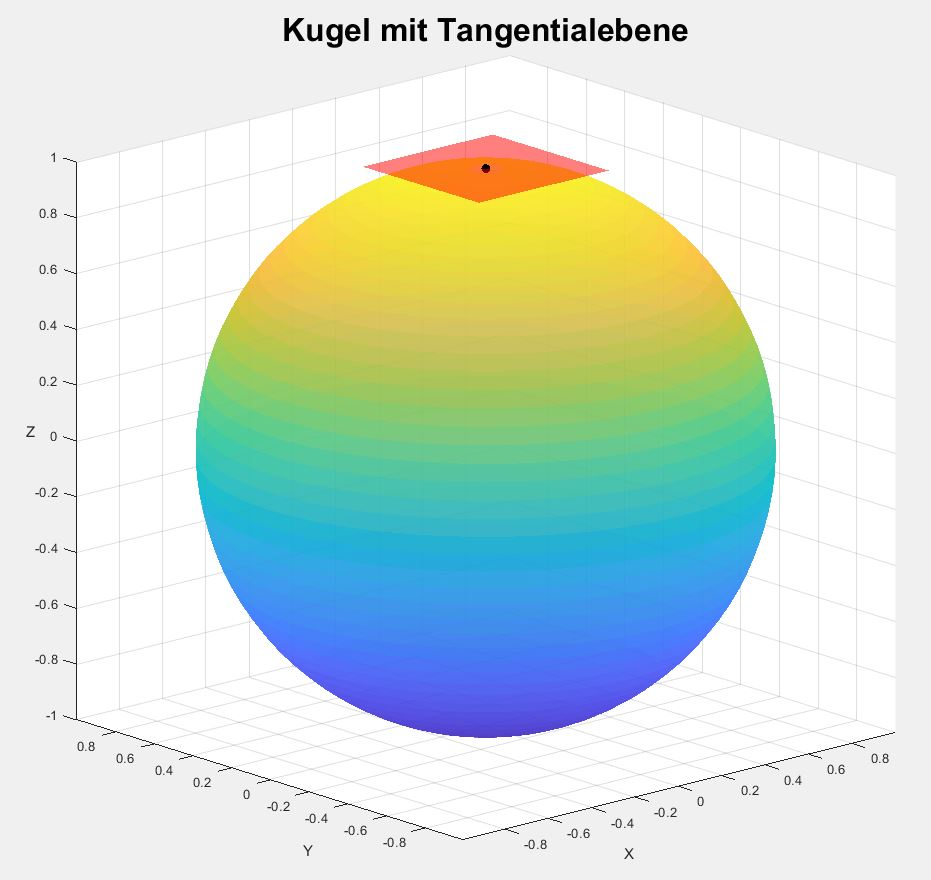
\includegraphics[width=1\linewidth]{papers/geodaeten/Abbildungen/MetrischerTensor/Tangentialebene}
	\caption{Tangentialebene eines Punktes der riemannschen Mannigfaltigkeit einer Kugeloberfläche.}
	\label{geodaeten:figure:MetrischerTensor:Tangentialebene}
\end{figure}

\subsection{Metrik und metrischer Tensor}
Die Metrik ist das grundlegende Werkzeug, welches uns ermöglicht, Längen, Abstände und Winkel in einem Raum zu messen.
In einfachen geometrischen Räumen, wie dem euklidischen Raum, kennen wir die Metrik bereits als den Satz des Pythagoras.
Wir haben auch schon in Abschnitt \ref{geodaeten:section:Linienelemente:Beispiele} die Metrik in verschiedenen Koordinatensystemen angewendet, um Linienelemente auf unterschiedlichen Oberflächen zu berechnen.

Um die Metrik mathematisch darstellen zu können wird der metrische Tensor $g_{i\!j}$ eingeführt.
\index{Tensor!metrisch}%
\index{gij@$g_{ij}$}%
Dieser Tensor ist eine symmetrische $n \times n$-Matrix, wobei $n$ der Dimension des Raumes entspricht, welche die Metrik an jedem Punkt der Mannigfaltigkeit kodiert.
Er enthält alle Informationen darüber, wie Abstände und Winkel in einem Raum berechnet werden.
Auf diese Weise beschreibt der metrische Tensor die geometrische Struktur des gesamten Raumes.

Eine differenzierbare Mannigfaltigkeit, die an jedem Punkt durch einen metrischen Tensor definiert ist, wird als riemannsche Mannigfaltigkeit bezeichnet. Zusätzlich erfordert eine riemannsche Mannigfaltigkeit, dass der metrische Tensor selbst stetig differenzierbar und ausserdem noch positiv definit ist. 
Dies bedeutet, dass in riemannschen Mannigfaltigkeiten kein negativer Abstand existieren kann.

Mit dem metrischen Tensor kann ein allgemeines, von Koordinatensystemen unabhängiges Skalarprodukt zweier Vektoren $\vec{u}$ und $\vec{v}$ definiert werden als
\begin{equation}
	\vec{u} \cdot \vec{v} = g_{i\!j} \, u^i \, v^j.
\end{equation}
Die Notation des metrischen Tensors stammt aus der Tensoralgebra,
\index{Tensoralgebra}%
wobei die einsteinsche Summenkonvention eine Summierung über die Indizes $i$ und $j$ impliziert, welche die Dimensionen des Raumes durchlaufen.
\index{Summenkonvention, einsteinsch}%
\index{einsteinsche Summenkonvention}%
Die Komponenten der Vektoren $u^i$ und $v^j$ werden dabei durch den metrischen Tensor $g_{i\!j}$ gewichtet, wodurch sich eine Summe in der Form von
\begin{equation}
	g_{11} \, u_1 \, v_1 + g_{12} \, u_1 \, v_2 + \dots + g_{nn} \, u_n \, v_n
\end{equation}
ergibt.
Berechnet man nun mit dieser allgemeinen Definition das Skalarprodukt eines infinitesimalen Vektors mit sich selbst, erhält man
\begin{equation}
	ds^2 = g_{i\!j} \, du^i \, du^j.
	\label{geodaeten:equation:MetrischerTensor:AllgemeinesLinienelement}
\end{equation}
Somit lässt sich das Linienelement in einer allgemeinen Form ausdrücken, die mithilfe des metrischen Tensors zu einer koordinatenunabhängigen Funktion wird.

Der metrische Tensor ist daher von zentraler Bedeutung für das Verständnis der Geometrie eines Raumes und ist ein fundamentales Werkzeug in der Differentialgeometrie und der allgemeinen Relativitätstheorie. 
Er ermöglicht es uns, die Metrik eines Raumes in eine kompakte Schreibweise zu überführen und liefert die Grundlage für die Berechnung von Abständen und Winkeln in komplexeren geometrischen Strukturen.

Im nächsten Abschnitt wird anhand von Beispielen gezeigt, wie die Metrik von verschiedenen Koordinatensystemen, in die kompakte Form des metrischen Tensors überführt werden kann.

\section{Beispiele zum metrischen Tensor}

%
% teil1.tex -- Beispiel-File für das Paper
%
% (c) 2020 Prof Dr Andreas Müller, Hochschule Rapperswil
%
% !TEX root = ../../buch.tex
% !TEX encoding = UTF-8
%
\subsection{Kartesisch\label{geodaeten:section:MetrischerTensor:Kartesisch}}
\rhead{Metrischer Tensor Beispiele}

Der Metrische Tensor für einen zweidimensionalen kartesischen Raum kann aus der Gleichung \eqref{geodaeten:equation:MetrischerTensor:AllgemeinesLinienelement} des allgemeinen Linienelements hergeleitet werden.
Schreiben wir die einsteinsche-Summe für zwei Dimensionen aus ergibt sich
\begin{equation}
	ds^2 = g_{11}  du^1  du^1 + g_{12}  du^1  du^2 + g_{21}  du^2  du^1 + g_{22}  du^2  du^2 .
	\label{geodaeten:equation:MetrischerTensor:Kartesisch:EinsteinSumme}
\end{equation}

In dem kartesischen Raum gilt, $du^1 = dx$ und $du^2 = dy$ wobei zu beachten ist, dass bei der Einsteinschen Summenkonvention die Hochstele keiner Potenz sondern eines Index entspricht.
Aus Abschnitt \ref{geodaeten:section:Linienelemente:Kartesisch} kennen wir das Linienelement des Kartesischen Raums als

\begin{equation}
	ds^2 = dx^2 + dy^2 .
\end{equation}
Aus dem Linienelement können wir die Koeffizienten von 

\begin{equation}
du^1 du^1 = dx^2 \quad \text{und} \quad du^2  du^2 = dy^2 
\end{equation}
als $1$ herauslesen.
Die Koeffizienten für

\begin{equation}
du^1 \cdot du^2 = dx \cdot dy \quad \text{und} \quad du^2 \cdot du^1 = dy \cdot dx
\end{equation}
sind beide $0$.
In Gleichung \ref{geodaeten:equation:MetrischerTensor:Kartesisch:EinsteinSumme} ist zu erkennen, dass diese Koeffizienten den Werten im metrischen Tensor $g_{ij}$ entsprechen.
An den richtigen Stellen eingesetzt ergibt sich der metrische Tensor des kartesischen Raums zu

\begin{equation}
	\begin{aligned}
		g_{11} &= \textcolor{red}{1} \\
		g_{12} &= \textcolor{blue}{0} \\
		g_{21} &= \textcolor{darkgreen}{0} \\
		g_{22} &= \textcolor{magenta}{1} \\
		g_{ij} &= \begin{pmatrix} \textcolor{red}{1} && \textcolor{blue}{0} \\ \textcolor{darkgreen}{0} && \textcolor{magenta}{1} \end{pmatrix} .
	\end{aligned}
\end{equation}


%
% teil1.tex -- Beispiel-File für das Paper
%
% (c) 2020 Prof Dr Andreas Müller, Hochschule Rapperswil
%
% !TEX root = ../../buch.tex
% !TEX encoding = UTF-8
%
\subsection{Zylinder\label{geodaeten:section:MetrischerTensor:Zylinder}}
\rhead{Metrischer Tensor Beispiele}

Für die Zylinderoberfläche gilt $r$ als konstant und $u^1 = \phi$, $u^2 =z$ 
Vergleicht man die Einstein-Summe aus Gleichung \eqref{geodaeten:equation:MetrischerTensor:Kartesisch:EinsteinSumme} mit dem Linienelement der Zylinderoberfläche

\begin{equation}
	\begin{aligned}
	ds^2 &= g_{11} \cdot du^1 \cdot du^1 + g_{12} \cdot du^1 \cdot du^2 + g_{21} \cdot du^2 \cdot du^1 + g_{22} \cdot du^2 \cdot du^2 \\
	&= r^2 \cdot d \phi^2 +dz^2
	\end{aligned}
\end{equation}
Kann mittels Koeffizienten Vergleich bestimmt werden, dass 

\begin{equation}
	\begin{alignedat}{3}
		g_{11} \cdot du^1 \cdot du^1 &= g_{11} \cdot d \phi^2 & &= r^2 \cdot d \phi^2 \\
		g_{22} \cdot du^2 \cdot du^2 &= g_{22} \cdot dz^2    & &= 1 \cdot dz^2 \\
		g_{12} \cdot du^1 \cdot du^2 &= g_{12} \cdot d \phi \cdot dz & &= 0 \cdot d \phi \cdot dz \\
		g_{21} \cdot du^2 \cdot du^2 &= g_{21} \cdot dz \cdot d \phi & &= 0 \cdot dz \cdot d \phi .
	\end{alignedat}
\end{equation}
Die Matrixeinträge entsprechen den Koeffizienten der jeweiligen Ableitungsprodukte und damit lässt sich der metrische Tensor aufstellen als
\begin{equation}
	g_{ji} =\begin{pmatrix} g_{11} && g_{12} \\ g_{21} && g_{22} \end{pmatrix}= \begin{pmatrix} r^2 && 0 \\ 0 && 1 \end{pmatrix} .
\end{equation}

Ist $r$ nicht konstant, bedeutet dies, dass man sich in drei Dimensionen bewegen kann.
Deshalb muss eine $3 \times 3$-Matrix für den metrischen Tensor entstehen, damit jede Bewegung vollständig beschrieben ist. 

Die Einstein-Summe hat hier die Form

\begin{equation}
\begin{aligned}
	ds^2 = &\ g_{11} \cdot du^1 \cdot du^1 + g_{12} \cdot du^1 \cdot du^2 + g_{13} \cdot du^1 \cdot du^3 \nonumber \\
	&+ g_{21} \cdot du^2 \cdot du^1 + g_{22} \cdot du^2 \cdot du^2 + g_{23} \cdot du^2 \cdot du^3 \nonumber \\
	&+ g_{31} \cdot du^3 \cdot du^1 + g_{32} \cdot du^3 \cdot du^2 + g_{33} \cdot du^3 \cdot du^3  .
\end{aligned} 
	\label{geodaeten:equation:MetrischerTensor:Kartesisch:EinsteinSumme3D}
\end{equation}

Im Linienelement des Zylinders aus \eqref{geodaeten:equation:Linienelemente:Zylinder:Zylinder3D} kann man herauslesen, dass keine Terme mit gemischten Ableitungsprodukte vorhanden sind.
Daher sind alle Einträge außer den Diagonalen Null.
Mit $u^1 = r$, $u^2 = \phi$ und $u^3 = z$  können die diagonalen Elemente mit den Koeffizienten im Linienelement bestimmt werden. 
Somit gilt,

\begin{equation}
	\begin{aligned}
		g_{11}  &= 1  \\
		g_{22}  &= r^2 \\
		g_{33}  &= 1  
	\end{aligned}
\end{equation}
und damit ist der metrische Tensor im dreidimensionalen zylindrischen Raum

\begin{equation}
	T = \begin{pmatrix} 1 && 0 && 0 \\ 0 && r^2 && 0 \\ 0 && 0 && 1 \end{pmatrix} .
\end{equation}

Dieses Beispiel veranschaulicht, dass der metrische Tensor eine $n \times n$-Matrix ist, wobei $n$ der Anzahl Dimensionen entspricht.
Dieser metrische Tensor beinhaltet eine Variable $r$ und ist somit nicht konstant. 
Daher existiert für die dreidimensionale Oberfläche des vierdimensionalen zylindrischen Raums eine Krümmung.
Diese Krümmung eines vierdimensionalen Raums ist allerdings schwer vorzustellen, weshalb die Krümmung des metrischen Tensors im Beispiel der Kugel (Abschnitt \ref{geodaeten:section:MetrischerTensor:Kugel}) genauer vorgestellt wird.

%
% teil1.tex -- Beispiel-File für das Paper
%
% (c) 2020 Prof Dr Andreas Müller, Hochschule Rapperswil
%
% !TEX root = ../../buch.tex
% !TEX encoding = UTF-8
%
\subsection{Kugel\label{geodaeten:section:MetrischerTensor:Kugel}}
\rhead{Metrischer Tensor Beispiele}

Sed ut perspiciatis unde omnis iste natus error sit voluptatem
accusantium doloremque laudantium, totam rem aperiam, eaque ipsa
quae ab illo inventore veritatis et quasi architecto beatae vitae
dicta sunt explicabo.
Nemo enim ipsam voluptatem quia voluptas sit aspernatur aut odit
aut fugit, sed quia consequuntur magni dolores eos qui ratione
voluptatem sequi nesciunt





%
% einleitung.tex -- Beispiel-File für die Einleitung
%
% (c) 2020 Prof Dr Andreas Müller, Hochschule Rapperswil
%
% !TEX root = ../../buch.tex
% !TEX encoding = UTF-8
%
\section{Differentialgleichung für Geodätenlinien
\label{geodaeten:section:Standardverfahren}}
\rhead{Differentialgleichung für Geodätenlinien}

Mit den Linienelementen und dem metrischen Tensor kann nun das Funktional für die Variation
\begin{equation}
	L = \int_T \sqrt{g_{ij} \dot{u}^i \dot{u}^j} dt
\end{equation}

als integral des zu minimierenden Weges aufgestellt werden.
Das verwenden des Raum spezifischen metrischen Tensors ermöglicht, diese allgemeine Formel für jede Art von Raum anzuwenden.
Daher der Name Standardverfahren.
Die Herleitung der Differentialgleichung ist hier zweitrangig und zunächst soll sie mittels einiger Beispiele veranschaulicht werden (Abschnitt \ref{geodaeten:section:StandardverfahrenBeispiele}).
Daher hier die Lösung des Funktionales, ohne Herleitung, welche die Geodäten-Differentialgleichung
\begin{equation}
	\ddot{u}^k + \Gamma_{ij}^k \dot{u}^i \dot{u}^j = 0 ,
	\label{geodaeten:equation:Standardverfahren:Geodaetengleichung}
\end{equation}

ergibt.
Diese allgemeine Geodätengleichung kann schließlich nach der Funktion des kürzesten Weges $u(t)$ aufgelöst werden.

Die Geodätengleichung beinhaltet die Christoffel-Symbol $\Gamma_{ij}^k$, welche mithilfe des metrischen Tensors berechnet werden können als
\begin{equation}
	\Gamma_{ij}^k = \frac{1}{2} g^{kl} \left( \frac{\partial g_{jl}}{\partial u^i} + \frac{\partial g_{il}}{\partial u^j} - \frac{\partial g_{ij}}{\partial u^l} \right) .
	\label{geodaeten:equation:Standardverfahren:Christoffel-Symbol}
\end{equation}

Die Christoffel-Symbol beschreiben, wie sich ein Raum in die Richtung einer Dimension ändert.
Der kürzeste Weg ist immer eine Gerade.
Für unterschiedlichen Räume hat eine Gerade jedoch immer eine andere Form.
Die Christoffel-Symbol können als Korrekturfaktor der geraden, abhängig vom Raum interpretiert werden.
Mit den Christoffel-Symbol können außerdem Aussagen über die Krümmung eines Raumes gemacht werden.
Sind die Christoffel-Symbol gleich Null herrscht im zugehörigen Raum keine Krümmung. 
Eine Gerade bleibt eine Gerade (Abschnitt \ref{geodaeten:section:StandardverfahrenBeispiele}).

\section{Beispiele zu den Differentialgleichungen für Geodätenlinien 
\label{geodaeten:section:StandardverfahrenBeispiele}}

%
% einleitung.tex -- Beispiel-File für die Einleitung
%
% (c) 2020 Prof Dr Andreas Müller, Hochschule Rapperswil
%
% !TEX root = ../../buch.tex
% !TEX encoding = UTF-8
%
\subsection{Kartesisch\label{geodaeten:section:Standardverfahren:Kartesisch}}
\rhead{Standardverfahren Beispiele}

\documentclass{article}
\usepackage{amsmath}
	
Für den kartesischen Raum mit dem metrischen Tensor 
\begin{equation}
g_{ij} = \begin{pmatrix} 
	1 & 0 \\ 
	0 & 1 
\end{pmatrix},
\end{equation}

wollen wir die Christophsymbole berechnen.
Die Christophsymbole sind gegeben durch,
\begin{equation}
\Gamma^i_{jk} = \frac{1}{2} g^{im} \left( \frac{\partial g_{mj}}{\partial x^k} + \frac{\partial g_{mk}}{\partial x^j} - \frac{\partial g_{jk}}{\partial x^m} \right),
\end{equation}

wobei $g^{im}$ die Inverse des metrischen Tensors ist.
Da der metrische Tensor $g_{ij}$ konstant ist und keine Abhängigkeit von den Koordinaten $\vec{x}$ hat, verschwinden alle Ableitungen.
Ohne weitere Berechnungen kann man also schließen, dass
\begin{equation}
\frac{\partial g_{ij}}{\partial x^k} = 0 .
\end{equation}

Somit ergeben sich alle Christophsymbole als null
\begin{equation}
\Gamma^i_{jk} = 0 .
\end{equation}

Denkt man an die Definition aus Abschnitt \ref{geodaeten:section:Standardverfahren}, macht dies durchaus Sinn.
Denn der Kartesische Raum ist nicht gekrümmt, weshalb keine Korrektur der Geraden notwendig ist.
Setzt man die Christophsymbole in die allgemeine Geodätengleichung ein erhält man mit $u^1 = x(t)$
\begin{equation}
\begin{aligned}
&\ddot{u}^1 + \Gamma_{ij}^1 \dot{u}^i \dot{u}^j = 0 \\
&\ddot{u}^1 + 0_{ij} \cdot \dot{u}^i \dot{u}^j = 0\\
&\ddot{u}^1 = 0 \\
&\ddot{x}(t) = 0
\end{aligned}
\label{geodaeten:equation:Standardverfahren:Kartesisch:x}
\end{equation}

und mit $u^2 = y(t)$

\begin{equation}
\begin{aligned}
&\ddot{u}^2 + \Gamma_{ij}^2 \dot{u}^i \dot{u}^j = 0 \\
&\ddot{u}^2 + 0_{ij} \cdot \dot{u}^i \dot{u}^j = 0 \\
&\ddot{u}^2 = 0 \\
&\ddot{y}(t) = 0 \qquad \qquad .
\end{aligned}
\label{geodaeten:equation:Standardverfahren:Kartesisch:y}
\end{equation}

Man sieht bereits, da die zweite Ableitungen in beide Dimensionen Null sind, handelt es sich bei dem Kürzesten Weg um eine Gerade.
Da sind wir froh, denn das macht durchaus Sinn.

Setzt man nun Zwei Punkte als Start und Endpunkt, kann man durch diese Nebenbedingungen eine konkrete Lösung erhalten.
Beispielsweise wollen wir den kürzesten Weg zwischen $P_A = (1,1)$ und $P_B = (3,5)$ berechnen. Wir integrieren die zweite Ableitung von x(t)

\begin{equation}
	\frac{d^2x}{dt^2} = 0 \Rightarrow \frac{dx}{dt} = c_1 
\end{equation}

, wobei $c_1$ eine Integrationskonstante ist. Durch erneutes Integrieren erhalten wir
\begin{equation}
\Rightarrow x(t) = c_1 \cdot t + c_2  .
\label{geodaeten:equation:Standardverfahren:Kartesisch:equation1}
\end{equation}

Wieder ist $c_2$ eine Integrationskonstante. 
Wir sehen, die Gleichung entspricht einer parametrierten Geradengleichung mit $c_2$ als Startwert für $x(0)$ und $c_1$ als Steigung von $x(t)$.

\begin{equation}
	P_A(x_1,y_1) \text{und} P_B(x_2,y_2)\\
	x(t) = (x_2 - x_1) \cdot t + x_1\\
	y(t) = (y_2 - y_1) \cdot t + y_1
\end{equation}

Da die Linie durch den Startpunkt gehen muss ist der Startwert bei $t=0$ bekannt als
 
\begin{equation}
	0 \cdot c_1 + c_2 = 1
\end{equation}
	
\begin{equation}	
	c_2 = 1 .
\end{equation}

Die Steigung $c_1$ kann mithilfe von Endpunkt und Startpunkt berechnet werden als

\begin{equation}
	c_1 = x_2 - x_1 \\ = 3-1 \\ = 2
\end{equation}

und damit ist die Lösung der Geodätengleichung in $x$ gleich

\begin{equation}
	x(t) = 2t + 1 .
\end{equation}


Analog für $y(t)$ ist [\ref{geodaeten:equation:Standardverfahren:Kartesisch:equation1}]
  
\begin{equation}
	\Rightarrow y(t) = c_3 \cdot t + c_4  .
\end{equation}

Die weiteren Gleichungen werden in $y(t)$ zu

\begin{equation}
	0 \cdot c_3 + c_4 = 1 
\end{equation}
 
\begin{equation}	
	c_4 = 1 .
\end{equation}

mit dem Einsetzen des Startwertes,

\begin{equation}
	c_4 = y_2 - y_1 \\=5-1 = 4
\end{equation}

mit der Steigung aus Sicht von $y$ und damit ist die Lösung der Geodätengleichung in $y$ gleich

\begin{equation}
	y(t) = 4t + 1 .
\end{equation}

\begin{figure}
	\centering
	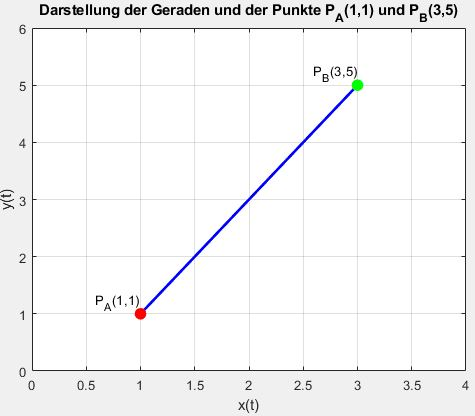
\includegraphics[width=10cm]{papers/geodaeten/Abbildungen/Standardverfahren/Kartesisch}
	\label{geodaeten:figure:Standardverfahren:Kartesisch:figure1}
	\caption{Darstellung der Kurve von x(t) und y(t) mit $t \in [0 , 1]$ Wie man sieht ist der kürzeste Weg von Punkt A zu Punkt B eine gerade.}
\end{figure}
%
% einleitung.tex -- Beispiel-File für die Einleitung
%
% (c) 2020 Prof Dr Andreas Müller, Hochschule Rapperswil
%
% !TEX root = ../../buch.tex
% !TEX encoding = UTF-8
%
\subsection{Zylinder\label{geodaeten:section:Standardverfahren:Zylinder}}
\rhead{Standardverfahren Beispiele}

Für die Zylinder Oberfläche mit konstantem $r$, mit dem metrischen Tensor 
\begin{equation}
	g_{ij} = \begin{pmatrix} 
		r^2 & 0 \\ 
		0 & 1 
	\end{pmatrix},
\end{equation}

wollen wir die Christophsymbole berechnen. 
Wie bei dem kartesischen Raum (Abschnitt \ref{geodaeten:section:Standardverfahren:Kartesisch}) werden alle Christophsymbole Null, da der metrische Tensor konstant ist.\footnote{
Auch in diesem Beispiel sind die Christophsymbole gleich Null.
Auf den ersten Blick könnte das verwirrend sein, da man bei einem Zylinder doch eindeutig eine Krümmung sieht.
Der Grund dafür ist, dass es sich bei dem Zylinder um eine extrinsische Krümmung handelt.
Die Zylinderoberfläche wird von außen zu einem Zylinder gekrümmt.
Abgerollt sieht man allerdings, dass die Oberfläche Flach ist.
Als weiteres Beispiel lässt sich berechnen, dass die Christophsymbole im Polarkoordinaten-Raum nicht gleich Null sind und daher eine Krümmung existiert, obwohl der Raum Flach erscheint.
Damit zeigt sich, dass die Intuition in diesem Fall täuschen kann.
}
Wir ersparen uns hier deshalb diese Rechnung.

Setzt man so $u^1 = \phi (t)$ und $u^2 = z(t)$ in die Geodätengleichung ein, so erhält man analog zu [\ref{geodaeten:equation:Standardverfahren:Kartesisch:x}]
\begin{equation}
	\ddot{\phi}(t) = 0
	\label{geodaeten:equation:Standardverfahren:Zylinder:phi}
\end{equation}

und dementsprechend gemäß [\ref{geodaeten:equation:Standardverfahren:Kartesisch:y}] 
\begin{equation}
	\ddot{z}(t) = 0 .
\end{equation}

Wählen wir $P_A(\phi_1 , z_1) = P_A(1 , 1)$ und $P_B(\phi_2 , z_2) = P_B(3 , 5)$ gleich wie in Abschnitt \ref{geodaeten:section:Standardverfahren:Kartesisch}, kennen wie bereits die Lösungen

\begin{equation}
	\phi(t) = 2t + 1 .
\end{equation}

\begin{equation}
	z(t) = 4t + 1 .
\end{equation}

Beim Zylinder ist jedoch interessant, dass es beliebige Lösungen für die Geodätengleichung gibt, da Die Winkelkoordinate Periodisch ist.
Durch Hinzufügen eines vielfachen von $2\pi$ macht die Kurve zusätzliche Runden um den Zylinder bevor es auf den Punkt $P_B$ trifft.
Dies ist zwar nicht die kürzeste Strecke, jedoch weder die Gleichung \ref{geodaeten:equation:Standardverfahren:Zylinder:phi} verletz noch der Punkt $P_a$ oder $P_B$ verfehlt.
Deshalb existieren sie als Scheinlösungen der Geodätengleichung.

Auch interessant ist, dass wenn die Oberfläche des Zylinders abgerollt auf eine Fläche dargestellt wird, ersichtlich ist, wie auch hier der kürzeste Weg eine Gerade ist.  

\begin{figure}
	\centering
	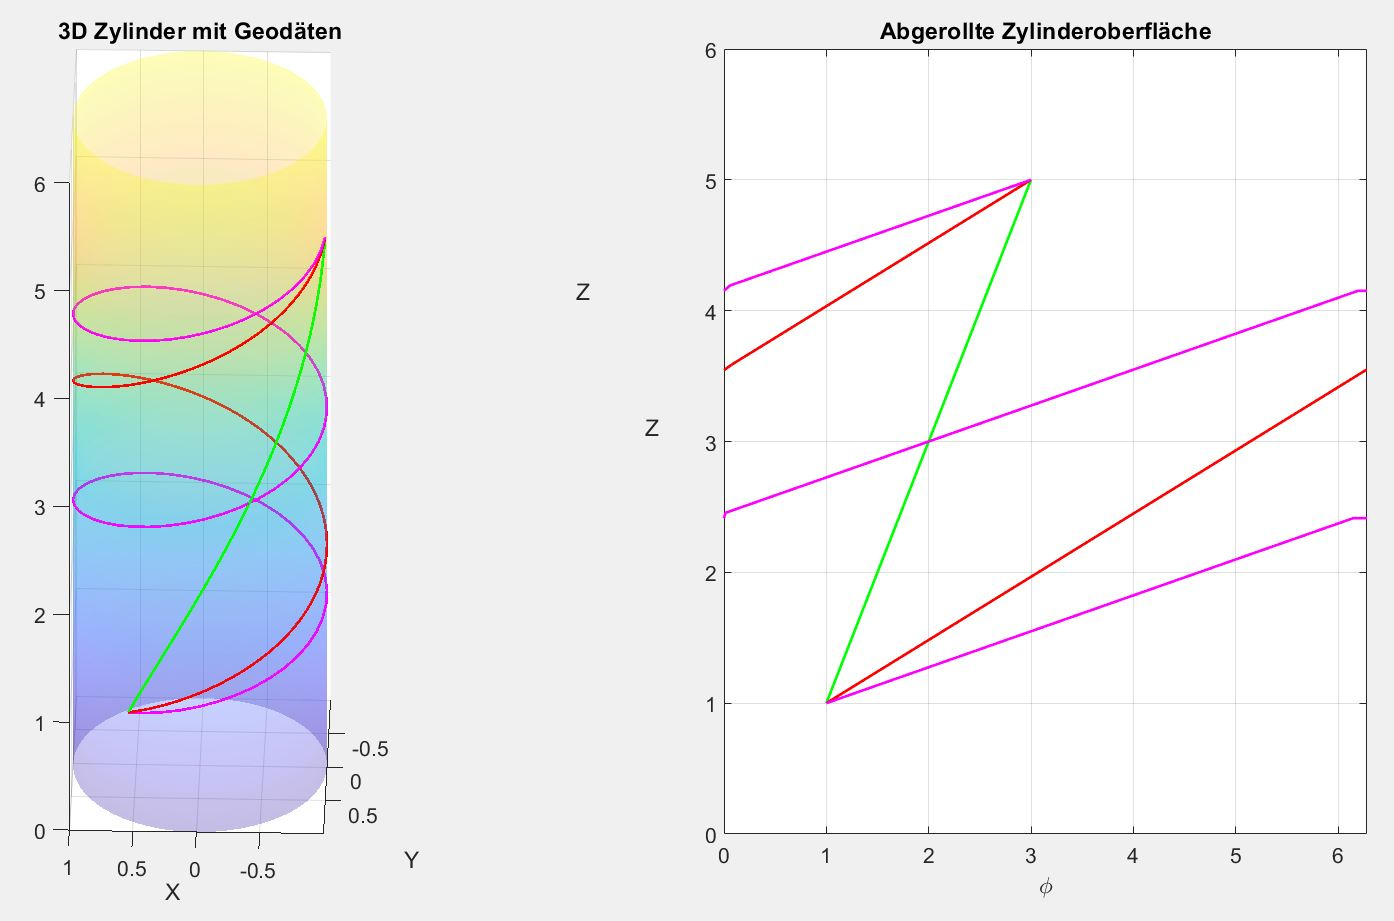
\includegraphics[width=14cm]{papers/geodaeten/Abbildungen/Standardverfahren/Zylinder}
	\caption{Darstellung der Geodätenlinien auf einem Zylinder und dessen abgerollte Oberfläche in einem 2D Plot mit Matlab}
	\label{geodaeten:figure:Linienelemente:Zylinder:figure1}
\end{figure}

%
% einleitung.tex -- Beispiel-File für die Einleitung
%
% (c) 2020 Prof Dr Andreas Müller, Hochschule Rapperswil
%
% !TEX root = ../../buch.tex
% !TEX encoding = UTF-8
%
\subsection{Kugel\label{geodaeten:section:Standardverfahren:Kugel}}
\rhead{Standardverfahren Beispiele}

Intuitiv erwarten wir, dass die Geodäten auf der Kugeloberfläche Grosskreise sind.
Ein Grosskreis ist der geradlinigste Weg zwischen zwei Punkten auf einer Kugel.
Dies kann man sich vorstellen, indem man zwei Nadeln in eine Kugeloberfläche steckt und einen Faden um die beiden Nadeln spannt.
Der Faden wird immer entlang eines Grosskreises verlaufen.
Tatsächlich folgen Flugzeuge auf Langstreckenflügen dieser Logik und fliegen entlang von Grosskreisen, um die kürzeste Strecke zwischen zwei Punkten auf der Erde zurückzulegen.
Wir möchten nun überprüfen, ob wir mit dem Standardverfahren tatsächlich zu dieser Lösung kommen.

Um dies zu tun, benötigen wir den bereits im vorherigen Abschnitt hergeleiteten metrischen Tensor für die Kugeloberfläche.
Dieser ist in Kugelkoordinaten $(\theta, \phi)$ gegeben durch
\begin{equation}
	g_{ij} = r^2 \begin{pmatrix}
		1 & 0 \\
		0 & \sin^2\theta
	\end{pmatrix}.
\end{equation}

Zuerst berechnen wir die Inverse des metrischen Tensors, da diese für die Berechnung der Christoffel-Symbol benötigt wird.
Der inverse Tensor $g^{ij}$ ist ergibt sich zu
\begin{equation}
	g^{ij} = \frac{1}{r^2} 
	\begin{pmatrix}
		1 & 0 \\
		0 & \frac{1}{\sin^2\theta}
	\end{pmatrix}.
	\label{geodaeten:equation:StaKugel:TensorInverse}
\end{equation}

Nun berechnen wir die partiellen Ableitungen des metrischen Tensors $g_{ij}$ in Bezug auf die Koordinaten $\theta$ und $\phi$.
Da $g_{11} = r^2$ und $g_{22} = r^2 \sin^2\theta$, erhalten wir
\begin{equation}
	\frac{\partial g_{11}}{\partial \theta} = 0, \quad \frac{\partial g_{11}}{\partial \phi} = 0, \quad \frac{\partial g_{22}}{\partial \theta} = 2r^2 \sin\theta \cos\theta, \quad \frac{\partial g_{22}}{\partial \phi} = 0.
	\label{geodaeten:equation:StaKugel:Ableitungen}
\end{equation}

\subsection{Christoffel-Symbole}
Mit den Ableitungen \eqref{geodaeten:equation:StaKugel:Ableitungen} und dem inversen Tensor $g^{ij}$ \eqref{geodaeten:equation:StaKugel:TensorInverse} können wir nun die Christoffel-Symbole berechnen durch
\begin{equation}
	\Gamma_{ij}^k = \frac{1}{2} g^{kl} \left( \frac{\partial g_{jl}}{\partial u^i} + \frac{\partial g_{il}}{\partial u^j} - \frac{\partial g_{ij}}{\partial u^l} \right),
\end{equation}
wobei $u^1 = \theta$ und $u^2 = \phi$.

Nach Einsetzen der Werte und Vereinfachung erhalten wir folgende nicht-verschwindende Christoffel-Symbole
\begin{equation}
	\Gamma_{12}^2 = \Gamma_{21}^2 = \cot\theta \quad \text{und} \quad \Gamma_{22}^1 = -\sin\theta \cos\theta.
\end{equation}

Anders als im Fall des Zylinders, wo der metrische Tensor konstant war, führt die Abhängigkeit des metrischen Tensors von der Koordinate $\theta$ zu nicht-verschwindenden Christoffel-Symbolen, welche die intrinsische Krümmung der Kugeloberfläche beschreiben.

Um diese Krümmung zu verstehen, betrachten wir die Bewegung eines Tangentialvektors auf der Oberfläche in Bezug auf die Basisvektoren.

Wird die Komponente des Vektors entlang eines Breitenkreises verändert, also in $\phi$-Richtung, führt das zu keiner Änderung der Vektorrichtung, da das Bogenmass von $\phi$ entlang eines Breitenkreises konstant bleibt.
Diese Bewegung beeinflusst die allgemeine Richtung des Vektors also nicht, was auch im metrischen Tensor reflektiert wird, der keinerlei Abhängigkeit von $\phi$ aufweist.

Andererseits führt eine Veränderung der Komponente entlang eines Längengrades, also in $\theta$-Richtung, zu einer Veränderung der Vektorrichtung.
Dies liegt daran, dass das Bogenmass von $\phi$ mit $\theta$ variiert: 
Je näher man den Polen kommt, desto kürzer wird der Bogen für eine gegebene Änderung von $\theta$, was die Gesamtrichtung des Vektors beeinflusst. 
Damit der Tangentialvektor seine ursprüngliche Richtung beibehält, müsste die Bewegung in der $\phi$-Richtung zunehmend verringert werden, je näher man den Polen kommt.

Diese Richtungsänderung des Vektors ist eine direkte Folge der intrinsischen Krümmung der Kugeloberfläche.
Die nicht-verschwindenden Christoffel-Symbole beschreiben genau diese Krümmung und geben an, wie sich die Richtung eines Vektors bei seiner Bewegung entlang der Oberfläche verändert.

\subsection{Geodätengleichung}
Mit den berechneten Christoffel-Symbolen können wir nun die Geodätengleichungen für die Kugeloberfläche aufstellen.

Die allgemeine Form der Geodätengleichung lautet
\begin{equation}
	\ddot{u}^k + \Gamma^k_{ij} \dot{u}^i \dot{u}^j = 0,
\end{equation}
wobei $u^k$ die Koordinaten darstellen, in diesem Fall $\theta$ und $\phi$.

Setzen wir die entsprechenden Christoffel-Symbole und Koordinaten in die Gleichungen ein, erhalten wir
\begin{equation}
	\begin{aligned} 
		0 &= \ddot{\theta} + \Gamma^1_{11} \dot{\theta} \dot{\theta} + 2\Gamma^1_{12} \dot{\theta}\dot{\phi} + \Gamma^1_{22} \dot{\phi} \dot{\phi} \\
		0 &= \ddot{\phi} + \Gamma^2_{11} \dot{\theta} \dot{\theta} + 2\Gamma^2_{12} \dot{\theta}\dot{\phi} + \Gamma^2_{22} \dot{\phi} \dot{\phi},
	\end{aligned}
\end{equation}
und weil einige der Christoffel-Symbole Null sind, vereinfachen sich die Geodätengleichungen schliesslich zu
\begin{align}
	0 &= \ddot{\theta} - \sin\theta \cos\theta \, \dot{\phi}^2 \\
	0 &= \ddot{\phi} + 2 \cot\theta \, \dot{\theta} \dot{\phi}.
\end{align}

Da $r$ lediglich ein Skalierungsfaktor ist, kürzt es sich in den Geodätengleichungen heraus. 
Die Geometrie wird allein durch die Winkelabhängigkeit bestimmt, sodass der Radius keinen Einfluss auf die Form der Geodäten hat.

Das Lösen der Geodätengleichungen ist oft aufwendig und schwierig, was numerische Ansätze erforderlich macht. 
Daher überprüfen wir durch Analyse, ob Grosskreise diese tatsächlich erfüllen und als Lösungen gelten.

\subsection{Äquator}
Betrachten wir die Geodätengleichungen für konstantes $\theta$, also entlang eines Breitengrads.
Für konstantes $\theta$ gilt $\dot{\theta} = 0$ und $\ddot{\theta} = 0$.
Setzen wir dies in die erste Geodätengleichung ein, so erhalten wir:
\begin{equation}
	0 = -\sin\theta \cos\theta \, \dot{\phi}^2.
\end{equation}
Die zweite Geodätengleichung vereinfacht sich zu $0 = \ddot{\phi}$, was zeigt, dass $\phi(t)$ linear in der Zeit variiert.
Diese erste Geodätengleichung wird nur für $\theta = \frac{\pi}{2}$ erfüllt, das heisst, nur für den Äquator.
Für alle anderen Breitengrade mit $\theta \neq \frac{\pi}{2}$ muss $\dot{\phi}$ gleich null werden, was bedeutet, dass es keine Bewegung in der $\phi$-Richtung gibt und somit keine Geodäte vorliegt.
Der Äquator, als einziger Breitengrad, erfüllt daher die Geodätengleichungen und ist ein Grosskreis.

\begin{figure}
	\centering
	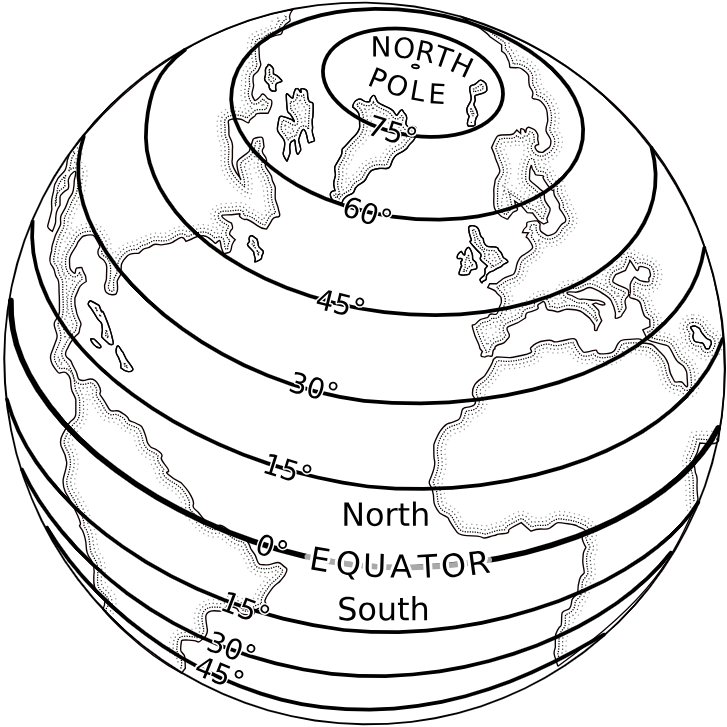
\includegraphics[width=1\linewidth]{papers/geodaeten/Abbildungen/Standardverfahren/StaKugelBreitengrade}
	\caption{Erdkugel mit Breitengrade und Äquator als Geodätenlinie}
	\label{geodaeten:figure:Standardverfahren:Breitengrade}
\end{figure}

\subsection{Längengrade}
Nun analysieren wir die Geodätengleichungen für konstantes $\phi$, also entlang eines Längengrads.
Für konstantes $\phi$ gilt $\dot{\phi} = 0$ und $\ddot{\phi} = 0$.
Setzen wir dies in die erste Geodätengleichung ein, erhalten wir:
\begin{equation}
	\ddot{\theta} = 0,
\end{equation}
was bedeutet, dass $\theta(t)$ linear in der Zeit variiert.
Die zweite Geodätengleichung wird ebenfalls trivial erfüllt, da $\dot{\phi} = 0$ und somit keine Beschleunigung in der $\phi$-Richtung vorliegt.
Damit sind alle Längengrade tatsächlich Geodäten.

Zusammenfassend konnten wir durch unsere Analyse zeigen, dass nur Grosskreise, wie der Äquator und die Längengrade, die Geodätengleichungen vollständig erfüllen und somit die wahren Geodäten auf der Kugeloberfläche darstellen.

Wir haben damit erfolgreich nachgewiesen, dass die Lösungen der Geodätengleichungen $\theta(t)$ und $\phi(t)$ zwangsläufig die Form von Grosskreisen annehmen müssen und dass die allgemeine Geodätengleichung diese Grosskreise korrekt als die Geodäten auf der Kugeloberfläche identifiziert.

\begin{figure}
	\centering
	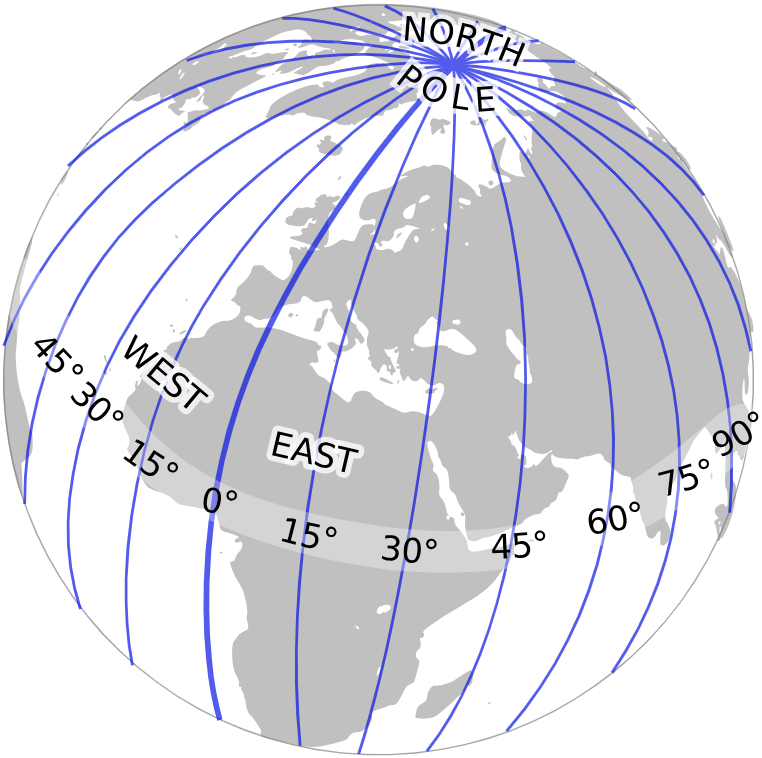
\includegraphics[width=1\linewidth]{papers/geodaeten/Abbildungen/Standardverfahren/StaKugelLaengengrade}
	\caption{Erdkugel mit Längengrade als Geodätenlinen}
	\label{geodaeten:figure:Standardverfahren:Laengengrade}
\end{figure}


\printbibliography[heading=subbibliography]
\end{refsection}
